%Data da última alteração:19/10/2016
\chapter{Trigonometria}
\begin{list}{\textbf{Questão \arabic{quest}.}}{\usecounter{quest}}
%define a margem da lista.	
%\setlength{\labelwidth}{-2mm} \setlength{\parsep}{0mm}
%\setlength{\topsep}{0mm} \setlength{\leftmargin}{-2mm}
\renewcommand{\labelenumi}{(\alph{enumi})}

\item Determine no triângulo retângulo ABC da figura o valor do seno, do cosseno e da tangente do ângulo agudo $\beta$. Considere $\sqrt{3}=3$
\begin{center}
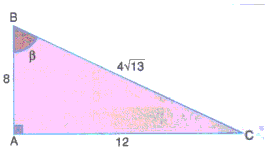
\includegraphics[scale=0.8]{figuras/fig84.png}
\end{center}

\item No triângulo retângulo da figura temos $tg\ \alpha=\displaystyle\frac{2}{3}$. Nessas condições, determine as medidas $x$ e $y$ indicadas.
\begin{center}
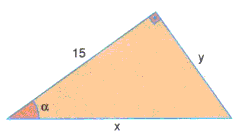
\includegraphics[scale=0.8]{figuras/fig85.png}
\end{center}

\item Determine a medida de x do cateto $AC$, no triângulo retângulo da figura. (Use: $sen\ 28º 
= 0,46$; $cos\ 28º = 0,88$ e $tg\ 28º = 0,53$)
\begin{center}
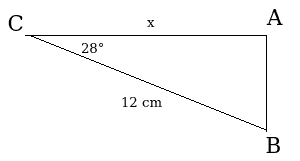
\includegraphics[scale=0.8]{figuras/fig86.png}
\end{center}


\item Encontre o valor do seno, cosseno e tangente do ângulo $\alpha$ nos triângulos retângulos a seguir.
\begin{multicols}{2}
\begin{enumerate}
	\item 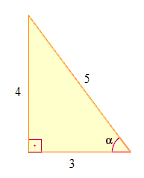
\includegraphics[scale=0.7]{figuras/fig87.png}
	\item 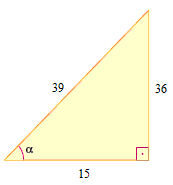
\includegraphics[scale=0.7]{figuras/fig88.png}
	\item 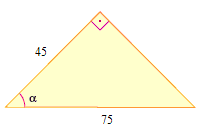
\includegraphics[scale=0.7]{figuras/fig89.png}
	\item 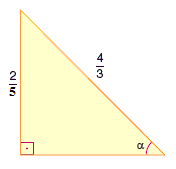
\includegraphics[scale=0.7]{figuras/fig90.png}
\end{enumerate}
\end{multicols}

\item Um garoto, curioso para saber a altura do prédio de um shopping, conseguiu com seu professor de Matemática um teodolito (tipo de instrumento de medição de ângulos) para auxiliá-lo nesse desafio. A situação é representada pela figura a seguir.
\begin{center}
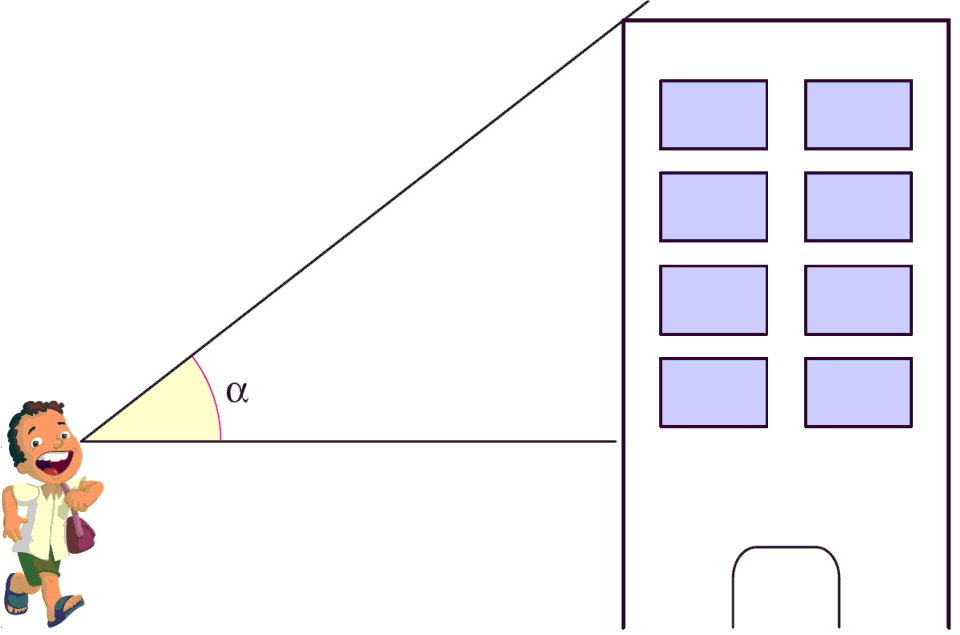
\includegraphics[scale=0.2]{figuras/fig91.png}
\end{center}
Suponha que a altura dos olhos do garoto com relação ao chão é de 1,50 m e que sua distância ao prédio do shopping é de 45 m. Sendo $tg\ \alpha = 2$, qual a altura do prédio?

\item Três amigos gostam de empinar pipa. Certo dia, com a pipa no ar, eles desenrolaram todo o carretel de linha, de 30 metros, conforme o desenho seguir.
\begin{center}
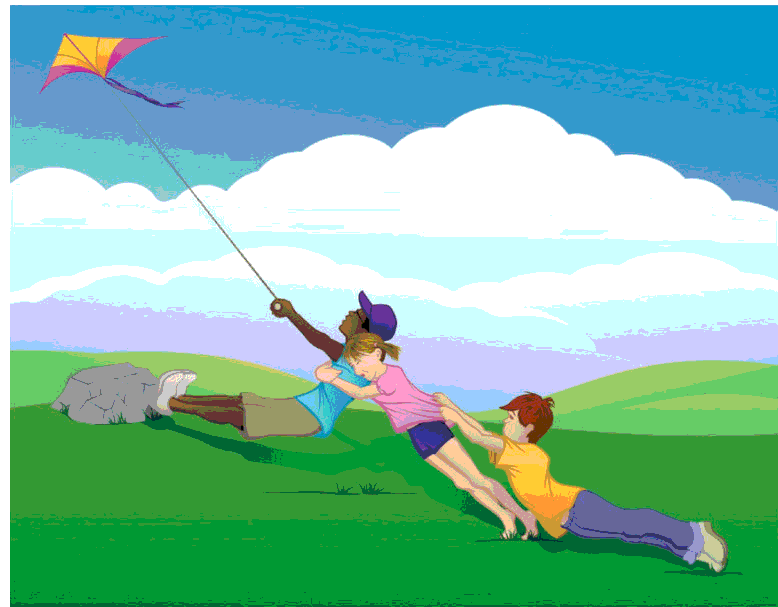
\includegraphics[scale=0.2]{figuras/fig92.png}
\end{center}
Sabendo que o seno do ângulo de inclinação da linha em relação ao solo é igual a 0,4, qual a altura aproximada da pipa?

\item Ao ancorar seu barco no Litoral Norte do estado de São Paulo, um pescador pode observar duas ilhas,A e B, como mostra a ilustração.
\begin{center}
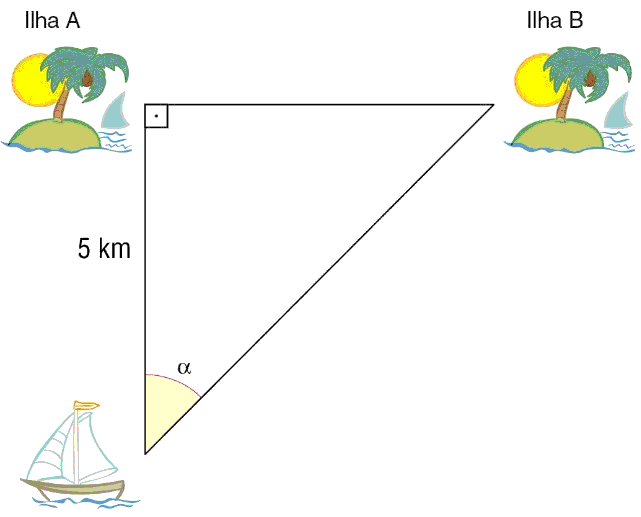
\includegraphics[scale=0.3]{figuras/fig93.png}
\end{center}
Qual a distância do barco do pescador em relação à ilha B? (use $cos\ \alpha = 0,8$).

\item Utilizando o seno dos ângulos indicados, encontre o valor de $x$.
\begin{multicols}{2}
\begin{enumerate}
	\item 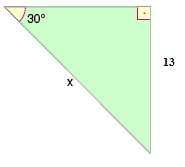
\includegraphics[scale=0.7]{figuras/fig94.png}
	\item 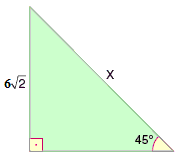
\includegraphics[scale=0.7]{figuras/fig95.png}
	\item 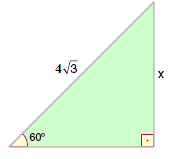
\includegraphics[scale=0.7]{figuras/fig96.png}
	\item 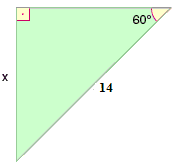
\includegraphics[scale=0.7]{figuras/fig97.png}
	\item 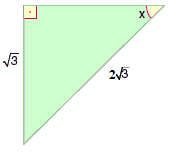
\includegraphics[scale=0.7]{figuras/fig98.png}
\end{enumerate}
\end{multicols}
\end{list}